%Toy example text
%\todo[inline]{I expect to see first the general control problem 13a-13e, then the specific example. This way, if you define once here, we dnot have to worry about re-defining the control problem later. So: here;s the general control problem; here's a simple system.}
%The control problem we solve is a version of \eqref{eq:min rob problem}, using the smooth version of robustness ($\srob$ instead of $\rob$).
%\begin{subequations}
%\label{eq:general_ctrl}
%\begin{align}
%\text{max } & \srob_{\formula}(\sstraj) - \gamma \sum_{k=0}^{N-1} l(x_{k+1},u_{k}) \\
%\text{s.t. } & x_{k+1} = f(x_k,u_k), \, \forall k=0,\dotsc,N-1 \\
% & x_k \in X, \, \forall k=0,\dotsc,N \\
% & u_k \in U, \, \forall k=0,\dotsc,N-1 \\
% & \delta \srob_{\formula}(\sstraj) \geq 0
%\end{align}
%\end{subequations}
%\todo[inline]{stick to $\formula$ for a formula, not $\formula$ (unless there's a good reason)}
%If we set $\gamma=0$ and $\delta=0$, we recover the problem in \eqref{eq:min rob problem} with the smooth robustness in the cost function. In the above formulation, $l(x_{k+1},u_{k})$ is a system specific control cost, e.g. the LQR cost $x_k'Qx_k + u_k'Ru_k$. $X$ and $U$ define constraints on the state $x$ and control $u$ respectively. 
To solve Problem $P_\rob$ given in \eqref{eq:general_ctrl}, we replace the true robustness $\robf$ by its smooth approximation $\srobf$.
We thus obtain Problem $P_{\srob}$.
We illustrate the approach on a simple linear system,
and provide more extensive case studies in Section \ref{sec:case study}.

\subsubsection{Illustrative example}
\label{sec:illustrative example}
We consider a linear system with the following dynamics:
\begin{equation}
\label{eq:PointMass}
x_{k+1} = x_k + u_k
\end{equation}

The specification is 
\[\formula = \always_{[0,20]} \neg (x_k \in \text{Unsafe}) \land \eventually_{[0,20]} (x_k \in \text{Terminal})\]
with the sets $\text{Unsafe}=[-1,1]^2$ i.e. a hyper-cube in $\mathbb{R}^2$ with length 2, centered on the origin) and $\text{Terminal}=[2,2.5]^2$. 
The state space is $X=[-2.5,2.5]^2$, $U=[0.3,0.3]^2$, $\delta=1$, and we optimize for two different values of $\gamma$, $0.1$ and $0.001$. 
The initial point of the optimization is $x_0=[-2,-2]'$. 
The control cost is $l(x_k,u_k) = ||x_k||_{2}^2$, so that $\sum_kl(x_k,u_k)$ penalizes the length of the trajectory. Here, $hrz(\formula) = 21$.

\textbf{Optimization solver.}
We use Sequential Quadratic Programming (SQP) to solve the optimization problem $P_{\srob}$.
SQP solves constrained non-linear optimization problems, like $P_{\srob}$, by creating a sequence of quadratic approximations to the problem and solving these approximate problems.
SQP enjoys various convergence-to-(local)-minima properties, depending on the assumptions we place on the problem. 
See \cite[Section 2.9]{Polak97_Optim}.
For example, for SQP to converge to a strict local minimum (a minimum that is strictly smaller than any objective function value in an open neighborhood around it), it suffices that 
1) all constraint functions be twice Lipschitz continuously differentiable (which is true in our case), and 
2) at points in the search space that lie on the boundary of the inequality-feasible set (where the inequality constraints are satisfied with equality), there exists a search direction towards the interior of the feasible set that does not violate the equality constraints (the so-called Mangasarian-Fromowitz constraint qualification) \cite[Assumption 2.9.1]{Polak97_Optim}.
This is also true in our case since our equality constraints come from the dynamics and are always enforced for any $\mathbf{u}$.

\textbf{Solver initialization}.
To initialize SQP (i.e., give it a starting point for the optimization), we need an \textit{initial trajectory} that starts from $x_0$. We can obtain this initial trajectory:

 a) The standard way, by solving a feasibility linear program with constraints \eqref{eq:general ctrl dyn}-\eqref{eq:general ctrl U}. By definition, the solution to a feasibility program is a trajectory that simply satisfies the constraints without optimizing the objective. This is in general a computationally lightweight solution as the optimization being solved is a simple linear program.
 
 b) By randomly generating an input sequence (which respects the bounds on the input/states). Such a trajectory will be fast to generate and feasible w.r.t the dynamics but is unlikely to satisfy the specification on the system. 

Note, the initial trajectory is free to violate the specification (as it does in every example we study in this paper) and we only enforce that it needs to satisfy the dynamics and constraints of the system which we are controlling.

%In most cases, SQP solvers can also recover from infeasible starts, that is the initial trajectory can also violate the dynamics and constraints of the system, but at the cost of computation effort, hence we enforce the feasibility constraint on the initial trajectory.

\textbf{Results}.
Fig.~\ref{fig:toy control} shows the sets, initial trajectory (which is unsafe and has a robustness of $-1$), and two trajectories obtained by solving $P_{\srob}$ for two different values of $\gamma$ (with $\delta=0$). Both trajectories satisfy the specification $\formula$. Intuitively, the trajectories in Fig.\ref{fig:toy control} make sense, as for a higher value of $\gamma=0.1$ we get a shorter trajectory, which is closer to unsafe set, hence satisfies $\formula$ less robustly ($\rob_{\formula}=0.65$) and for a smaller value of $\gamma=0.001$ we get a longer trajectory with a higher robustness ($\rob_{\formula}=1.21$).

\textbf{Comparison to BluSTL.}
We also compare the timing and robustness maximization performance for our method with BluSTL \cite{}. BluSTL has two modes of operation, \textit{boolean}: which aims at satisfying the specification (we set control cost to zero), and \textit{robust}: which uses a MILP encoding of robustness and attempts to maximize it (again we set control cost to zero). For a fair comparison of our method to BluSTL, we emulate the \textit{boolean} mode of BluSTL by terminating the optimization at the iteration of SQP where $\srob \geq \epsilon_{\text{Meyer}}$. The \textit{robust} operation is obtained by solving $P_{\srob}$ until SQP terminates (on a local minima, possibly global). Similar to the optimization cost of BluSTL, we set $\gamma=0$ in $P_{\srob}$ for both modes, i.e. no control cost. All methods are run in a one-shot manner, that is a single optimization is solved at time step $0$ to get a trajectory with a length of $N$ time steps, where $hrz(\formula) = N$.

We run 100 instances with the specification and dynamics of our illustrative example, with a random initial state $x_0 \in [-2.5,-1.5] \times [-2.5,2.5]$ for each instance. We also vary the formula horizon (and hence optimization length of the trajectory being optimized over) $N$ from $20$ to $50$ time-steps in increments of 10. Table \ref{tbl:time_performance_toy} shows the $95^{th}$ percentile execution times for each method and the two modes of operation. All experiments were run on a machine with a quad-core Intel I5 3.2GHz processor with 24GB RAM, running MATLAB 2016b.


\begin{table}[tb]
\small
\begin{center}
\caption{{\small $95^{th}$ percentile runtimes (in seconds) for Smooth Operator (SOP) and BluSTL over 100 runs with random initial states and with different formula horizon lengths $N$. Here, (B) means \textit{boolean} mode and (R) means \textit{robust} mode of operation.}}
\vspace{-5pt}
\label{tbl:time_performance_toy}
\begin{tabular} {|c|c|c|c|c|}
	\hline
	N & BS(B) & SR-SQP(B) & BS(R) & SR-SQP(R) \\ \hline
	20 & 0.3213 &  \textbf{0.1211} & NA & 1.8249 \\ \hline
	30 & 0.5648 &  \textbf{0.1345} & NA & 2.6201\\ \hline
	40 & 0.8262 &  \textbf{0.3074} & NA & 5.7611\\ \hline
	50 & 1.9285  & \textbf{0.7394} & NA & 30.0574\\ \hline
\end{tabular}	
\end{center}
\end{table}

\textbf{Analysis.}
As seen in table \ref{tbl:time_performance_toy}, our SR-SQP performs faster than BluSTL. For BluSTL in \textit{robust} mode, BluSTL could not finish a single instance within 100 hours on both the machine used for running experiments as well as on a machine with 8 core Intel Xeon machine with 60GB RAM.
When in \textit{boolean} mode, BluSTL results in trajectories with zero robustness (as seen in), while our method results in trajectories with an average robustness of 0.10. Both methods satisfy $\formula$ in all 100 instances. In \textit{robust} mode, across all experiments, SR-SQP results in an average $\rob_{\formula}=0.247$ with a standard deviation of less than $0.005$. It is to be noted, that an upper bound on the maximum achievable $\rob_{\formula}$ is $0.25$, which can be achieved by trajectory reaching (in number of time steps $\leq N$) the point $[2.25,2.25]$ in the middle of the Terminal set while always avoiding the Unsafe set by a distance greater than $0.25$. This shows that for this particular problem, our method reaches very close to achieving the global optima of $\rob_{\formula}$.

\begin{figure}[t]
\centering
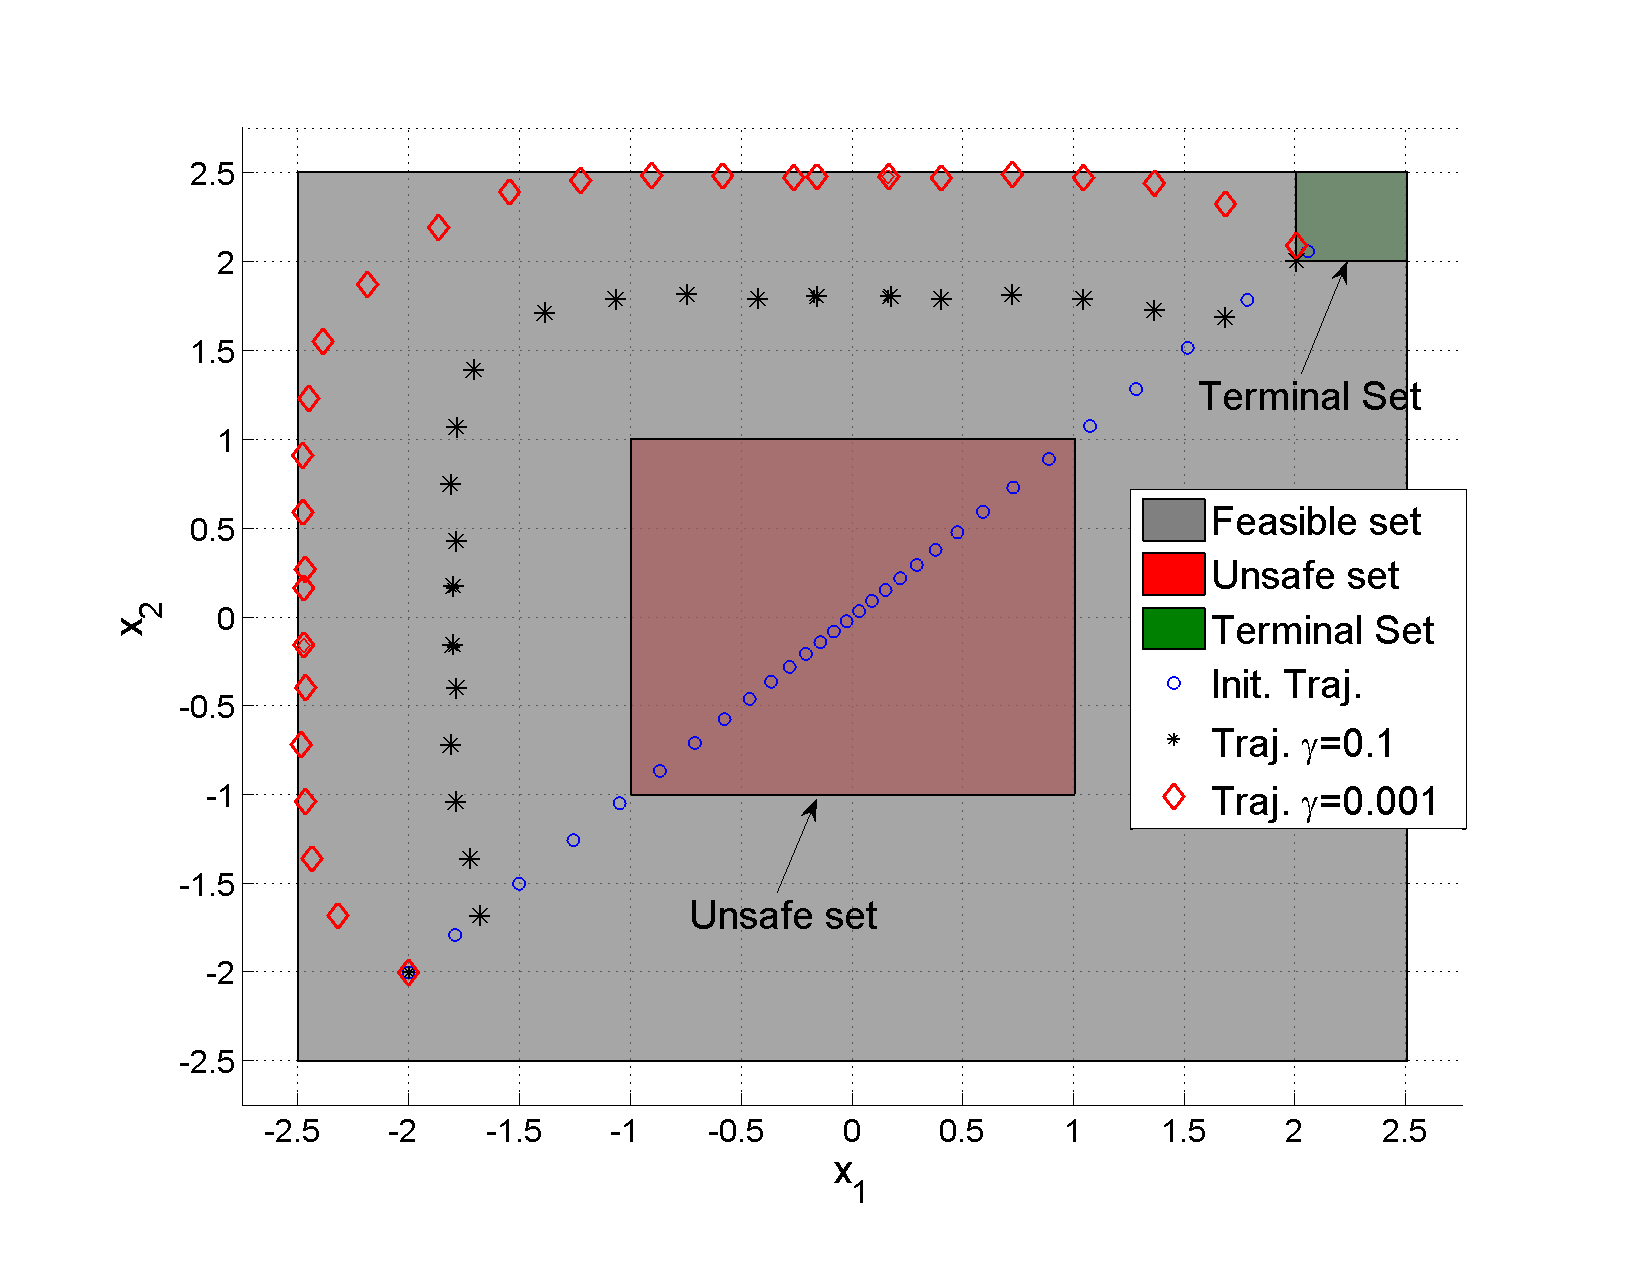
\includegraphics[width=0.49\textwidth]{figures/ToyExampleControl}
\vspace{-30pt}
\caption{{\small Initial trajectory and trajectories obtained for two different values of $\gamma$ in \eqref{eq:general_ctrl}.}}
\label{fig:toy control}
\vspace{-10pt}
\end{figure}